% chapter2.tex -- en (English)
\chapter{Operating Instructions}

This chapter is a classical operator's guide for users who intend to
use the {\Bezeichnung} straight forward without modifying the software 
or hardware of the device.


\section{Power On}
To switch on the {\Bezeichnung}, set the mains switch at the back of the
unit to position I. The boot process of the Raspberry Pi will start and
the operating system on the SD card (Raspbian Stretch Desktop from
13-03-2018) is loaded to the main memory. After approx. 10 seconds the 
boot process is completed and the desktop appears on the display (see 
figure \ref{fig:desktop00}).

\begin{figure}[h]
\centering
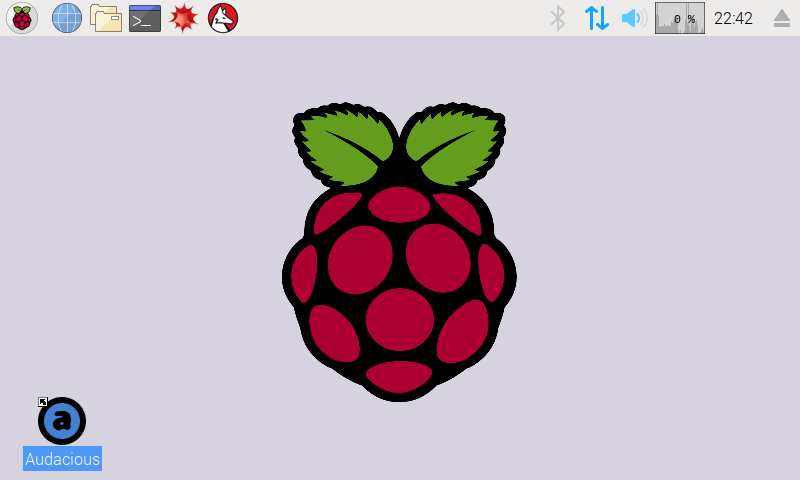
\includegraphics[width=0.8\textwidth]{desktop00.png}
\caption{Raspbian Stretch Desktop}
\label{fig:desktop00}
\end{figure}


\section{Secure Shut Down and Power Off}
To avoid data corruptions please shut down the {\Bezeichnung} securely!
First, shut down the operating system (Raspbian Stretch Desktop) via the
menu item \menuitem{\rpiIcon$\rightarrow$Shutdown...$\rightarrow$Shutdown}.
After the display has turned black, wait again for approx. 10 seconds 
before switching off the power via the mains switch on the back of the 
unit.

\begin{figure}[h]
\centering
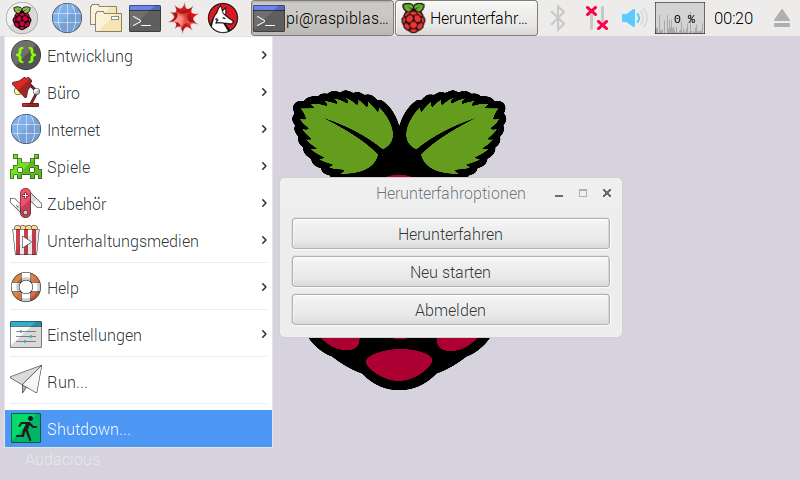
\includegraphics[width=0.8\textwidth]{\lang/desktop08.png}
\caption{Shut Down {\Bezeichnung}}
\label{fig:desktop08}
\end{figure}

\begin{bclogo}[arrondi = 0.2, logo = \bcinfo, ombre = true, epOmbre = 0.25, couleurOmbre = black!30,blur]{Caution}
Take care to shut down the {\RPi} completely before switching off the
power supply! If the power supply is removed \textit{exactly} when the
device is performing a write access to the SD card, this write access
may be incomplete or incorrect and may damage the file system on the SD
card in an undefined way. Though in most cases this won't happen, avoid
switching off the mains power without shutting down to prevent data loss
on the SD card.
\end{bclogo}


\section{Volume Control}
The taskbar of Raspbian shows a speaker icon in the upper right corner.
Clicking this icon will open a graphical slider control that can be used
to adjust the playback volume. The set current volume is roughly 
indicated by symbolic acoustic waves (1 -- 3) in front of the speaker 
icon. A red \textcolor{red}{\texttt{x}} means muting of the audio 
reproduction.


\section{Starting the Audio Player \audacious}
The software {\audacious} -- {\audaciousStable} is used to play CDs on 
the {\Bezeichnung}. To start this software use either the menu item
\menuitem{\rpiIcon$\rightarrow$Sound \& Video$\rightarrow$Audacious}
or double-click on the ``Audacious'' icon at the bottom left 
corner of the desktop.


\section{Insert CD and Start Playback}
Open the CD drive using the eject push button and insert the CD to play 
(see figure \ref{fig:insertCD}). Close the CD tray manually.

\begin{figure}[h]
\centering
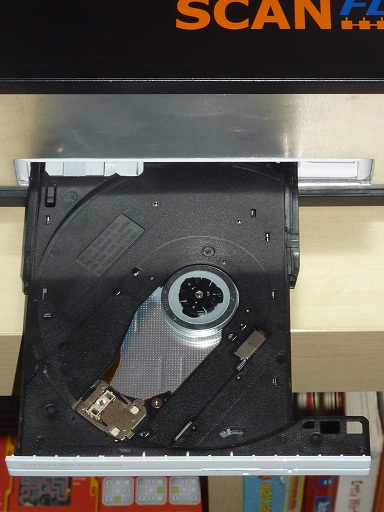
\includegraphics[width=0.4\textwidth]{tray_empty.jpg}
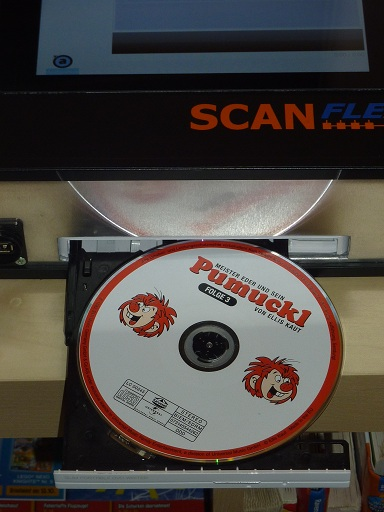
\includegraphics[width=0.4\textwidth]{tray_CD.jpg}
\caption{Insert CD into Tray}
\label{fig:insertCD}
\end{figure}

The drive needs a short time to read the table of contents of the CD.
Raspbian will show the system dialogue box \dialogbox{Removable medium 
is inserted}. Now the CD is ready for playback. This dialogue box can
be closed by clicking the button \button{Cancel}. 

\begin{figure}[h]
\centering
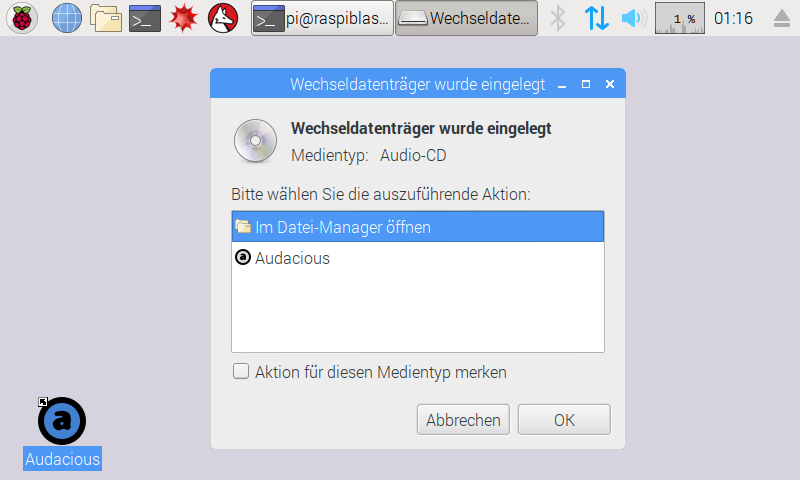
\includegraphics[width=0.8\textwidth]{\lang/desktop09.png}
\caption{System Dialogue Box ``Removable medium is inserted''}
\label{fig:desktop09}
\end{figure}

To start the playback of the inserted CD use {\audacious}' menu item
\menuitem{Services$\rightarrow$Play CD}. {\audacious} inserts all tracks
of the CD into a playlist named ``Now Playing''. If this playlist is
already containing some entries all these entries will be removed and
replaced by the tracks of the current CD! See section \ref{sect:playlist}
for details. CDs following the first version of the CDDA specification
are lack of any meta data like song title, artist ect. Thus the playlist
will be filled with denominations like ``Track <x>'' and the album name
``Audio CD''. Most of newer CDs contain meta data in the format 
``CD-TEXT''. When reading such CDs the CD-TEXT information will be taken
into the playlist.

\begin{bclogo}[logo = \bclampe, noborder = true]{Hint}
To get automatically track information even for older CDs of the first 
generation, {\audacious} uses the internet database \textit{Compact Disc
Database} (CDDB) for receiving according meta data. The length of all
tracks of the CD is sent to CDDB. The CDDB server requests its data base
for meta data matching to the transmitted track lengths.\\
To use the feature of CDDB data base the {\Bezeichnung} has to be 
connected to the internet!\\
\url{https://de.wikipedia.org/wiki/CDDB}
\end{bclogo}


\section{Operating}
The graphical user interface of the audio player {\audacious} provides
all controls which are known from a ``classical'' CD player.
\subsection*{Play/Pause}
Starting and pausing playback
\subsection*{Skip |<<}
Select previous track
\subsection*{Skip >>|}
Select next track
\subsection*{Rewind and fast forward}
Rewinding and forwarding of a track is done in  {\audacious} by moving
the current position of the track progress bar.
\begin{bclogo}[logo = \bclampe, noborder = true]{Hint} 
This method allows really fast jumps to a certain position (or the 
beginning) of a track. So the button \textit{Skip |<<} jumps 
\textbf{always} to the previous track. This is in contrast to many CD 
players where you might expect a jump to the beginning of the currently 
playing track.
\end{bclogo}
\subsection*{Stop}
Stop playback
\subsection*{eject}
Opens the CD tray of the drive
\begin{bclogo}[logo = \bclampe, noborder = true]{Hint}
The feature \textit{eject} was added by {\autor} to the {\RPi} version
of {\audacious} for {\Bezeichnung}.
\end{bclogo}


\section{Playlist}
\label{sect:playlist}
{\audacious} manages all tracks to play in so-called playlists. This is
ideal for creating long compilations of audio files stored on external
storage devices like USB flash drives. {\audacious} is able to provide 
more than one play list at a time to sort the music by genres like
Heavy Metal, Classics, Rap, Folk. The playback of tracks is given by the
currently active playlist.
\begin{bclogo}[logo = \bclampe, noborder = true]{Hint} 
When starting CD playback via the menu item 
\menuitem{Services$\rightarrow$Play CD} all tracks of the CD are 
inserted to the playlist ``Now Playing''. Old tracks in this special 
playlist will be removed! But after the automatic creaton of this list 
you may add further tracks from a USB drive or remove other tracks.\\
When changing the name of this playlist and starting a new CD playback
by the menu item \menuitem{Services$\rightarrow$Play CD} a new playlist
called ``Now Playing'' will be created again.
\end{bclogo}


\section{Playback of Audio Files On Other Storage Media}
{\audacious} is compatible to a lot of audio formats like MP3 or FLAC
which may be stored on a {\CDROM} or a USB flash drive. Even audio files 
stored on the SD card of the {\RPi} can be used.\\
When loading video files {\audacious} only plays their audio track.


\section{Handling and Cleaning of CDs}
\begin{compactitem}
\item{Grab the CD always at its edge to keep it clean}
\item{Don't stick paper or tape on the CD's surface}
\item{Protect CDs from heat:\\Keep them away from direct sun light and heating devices. Don't leave them in a car parking in the sunshine}
\item{Always store the CD in its sleeve after listening.}
\end{compactitem}

\begin{figure}[h]
\centering
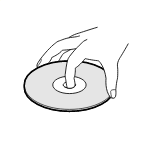
\includegraphics[width=0.3\textwidth]{CD_handling.png}
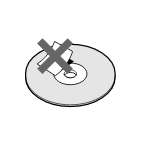
\includegraphics[width=0.3\textwidth]{CD_no_labels.png}
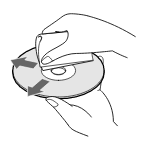
\includegraphics[width=0.3\textwidth]{CD_cleaning.png}
\caption{Handling of CDs}
\label{fig:CDhandling}
\end{figure}

\begin{compactitem}
\item{Clean the CD with a lint-free cleaning cloth, wiping from the inside out.}
\item{Do not use solvent-containing cleaning agents such as petrol or thinner.}
\end{compactitem}


\newpage
\section{Error Handling}
If the device behaves incorrectly, first check whether the error can be
corrected with simple means. Especially systems on which complex 
software (\eg the operating system Raspbian or {\audacious}) is running,
are highly configurable and not any unexpected behavior is really an
error but can often be eliminated by simple measures.\\
The following list is not exhaustive:

\subsection{{\Bezeichnung} doesn't boot}
\begin{compactitem}
\item{The SD card is not inserted correctly (anymore).}
\item{The file system on the SD card was damaged by incorrect power off}
\item{Fundamental files on the SD card have been deleted or moved}
\end{compactitem}
Each reason makes it necessary to open the case of {\Bezeichnung} for 
removing the {\RPi}'s SD card, because the {\RPi} cannot boot from it.
The SD card has to be corrected or reloaded on an external PC!

{\begin{bclogo}[arrondi = 0.2, logo = \bcdanger, ombre = true, epOmbre = 0.25, couleurOmbre = red!75,blur]{Danger!} 
Due to the risk of a dangerous electric shock remove mains plug before 
opening the case!\\
\end{bclogo}


\subsection{The eject push button of the {\CDROM} drive doesn't work}
\begin{compactitem}
\item{During playback of a CD the eject push button is locked} 
\end{compactitem}
Before ejecting a CD the software button \button{Stop} in {\audacious} 
must be actuated to stop playback. This releases the hardware push 
button of the drive. 
\begin{bclogo}[logo = \bclampe, noborder = true]{Hint}
The software button \button{eject} of {\audacious} allows opening the
{\CDROM} drive at any time.
\end{bclogo}


\subsection{The screen is black}
\begin{compactitem}
\item{Is the screen saver active?\\
      Touch the display for activating it}
\item{Is the power supply working? Are the cables connected correctly?}
\item{Are the micro-fuses inside the mains switch OK?}
\end{compactitem}
Check the mains cord on tight connection.\\
Does the wall socket really supply mains voltage?\\
Check the micro-fuses in the {\Bezeichnung}. The device must always be 
fused on both poles!

{\begin{bclogo}[arrondi = 0.2, logo = \bcdanger, ombre = true, epOmbre = 0.25, couleurOmbre = red!75,blur]{Danger!} 
Before checking the micro-fuses remove the mains plug, even if the mains
switch is in position 0! When the fuse holder is open, there is the risk
of a dangerous electric shock from touching the contacts!
\end{bclogo}

\begin{bclogo}[arrondi = 0.2, logo = \bcinfo, ombre = true, epOmbre = 0.25, couleurOmbre = black!30,blur]{Caution}
When changing the micro-fuses take care of using new fuses of the same
type:\\
250V max, 1A slow blow\\
\end{bclogo}


\subsection{No Audio Signal}
\begin{compactitem}
\item{Is the volume set correct?\\
      A red-marked \textcolor{red}{\texttt{x}} on the speaker icon 
      indicates a muted playback.}
\item{Silent or complete mute part in the track?}
\item{Is the CD playing?}
\item{Are the audio sources (CD, USB drive) of the tracks in the playlist still available?}
\item{Is the CD erroneous or scratchy?\\
      A test with another CD is recommended}
\item{Using external speakers: Are the speakers connected correctly?\\
      Take a look on two topics:\\
      * correct cabling\\
      * correct position II of speaker switch on top of the {\Bezeichnung}\\
      Set speaker switch on position I to check if there is an audio 
      signal on the internal speakers.}
\end{compactitem}
